%%%--------------------------------%%%
%%% UC3
%%%--------------------------------%%%

\newpage
% UC3 ====================================================
\subsubsection{Use Case Specification: \ac{UC}3 Risk CRUD}
\label{sec:domainBbd}

\paragraph*{Description}\mbox{}\\
This use case allows users to create, read, update and delete risks. 
A risk consists of the following fields:
\begin{itemize}
	\vspace{-3mm}
	\setlength\itemsep{-1em}
	\item name (String)
	\item description (String)
\end{itemize}
Following fields are filled later and are not part of the input form:
\begin{itemize}
	\vspace{-3mm}
	\setlength\itemsep{-1em}
	\item probability of occurence (Enum)
	\item impact (Enum)
	\item risk factor (Enum)
	\item response (Objects)  
	\item person in charge (User)
	\item public risk (boolean)
\end{itemize}

\paragraph*{Screenshots}\mbox{}\\
tbd: Insert screenshots and shortly explain what can be seen
\begin{figure}[h] 
	\centering
	
\includegraphics[width=0.1\textwidth]{Content/Domain/placeholder.png}
	\caption{\ac{UC}3 Risk CRUD: TODO}
	\label{fig:label3}
\end{figure}

\newpage
\paragraph*{Basic Flow} \mbox{}\\
\noindent
Creating a risk:
\begin{itemize}
	\vspace{-3mm}
	\setlength\itemsep{-1em}
	\item  When the user clicks the "+" button at the project overview page.
	\item Then the screen for adding a new risk is opened.
	\item When the risk form is filled by the user.
	\item And the user clicks on the "Propose risk" button.
	\item Then the risk is synced with the server.
\end{itemize}

\noindent
Reading a risk:
\begin{itemize}
	\vspace{-3mm}
	\setlength\itemsep{-1em}
	\item The user is on the project overview site with all project risks.
	\item By clicking on a risk a detail risk view is opened.
	\item For exiting the risk detail view a return button ("Close" button) is clicked.
\end{itemize}

\noindent
Updating a risk: 
\begin{itemize}
	\vspace{-3mm}
	\setlength\itemsep{-1em}
	\item The user is on the project overview site with all project risks.
	\item By clicking on a risk a detail risk view is opened.
	\item On the detail view there is a pen button, enabling editing and changing the "Close" button to a "Save" button.
	\item When clicking the "Save" button the changes are syncronized with the server.
\end{itemize} 

\noindent
Deleting a risk:
\begin{itemize}
	\vspace{-3mm}
	\setlength\itemsep{-1em}
	\item The user is on the project overview site with all project risks.
	\item By clicking on a risk a detail risk view is opened.
	\item By clicking a "Delete" button the risk is deleted. This behavior is changed in UC6 Risk Discussion described in chapter \ref{sec:domainBbg}.
\end{itemize}

\newpage
\subparagraph{Activity Diagram}\mbox{}\\
\begin{figure}[H]
	\centering
	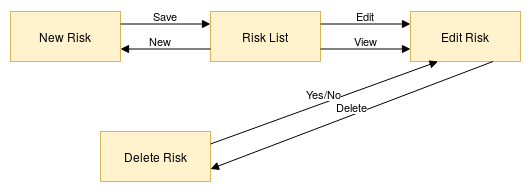
\includegraphics[width=0.9\textwidth]{Content/Domain/UC3RiskCRUDactivitydiagram.png}
	\caption{Activity Diagram \ac{UC}3 Risk CRUD}
	\label{fig:activityDiagramUC3}
\end{figure}

\paragraph*{Alternative Flows}\mbox{}\\
n/a

\paragraph*{Special Requirements and Preconditions}\mbox{}\\
The preconditions for this use case are:
\begin{enumerate}
	\vspace{-3mm}
	\setlength\itemsep{-1em}
	\item A project exists.
	\item The user is member of the project.
	\item The user has clicked the "+" button at the project overview page to add a new risk.
\end{enumerate}

\paragraph*{Postconditions and Persistance}\mbox{}\\
The postconditions for this use case are:
\begin{enumerate}
	\vspace{-3mm}
	\setlength\itemsep{-1em}
	\item The risk is immediately part of the projects risk table (this behavior is changed within UC6 Risk Discussion described in chapter \ref{sec:domainBbg}).
\end{enumerate}

\noindent
The persistence guidelines are: 
\newline
\noindent
The risk form was completely or partly filled by the user. When the user tries to leave the page now, there should be a prompt for exiting. When the risk form is filled out and the button "Propose risk" is clicked a POST request syncs the status with the server.
